\chapter{Design}



%You should concentrate on the more important aspects of the design. It is essential that an overview is presented before going into detail. As well as describing the design adopted it must also explain what other designs were considered and why they were rejected.

%The design should describe what you expected to do, and might also explain areas that you had to revise after some investigation.

%Typically, for an object-oriented design, the discussion will focus on the choice of objects and classes and the allocation of methods to classes. The use made of reusable components should be described and their source referenced. Particularly important decisions concerning data structures usually affect the architecture of a system and so should be described here.

%How much material you include on detailed design and implementation will depend very much on the nature of the project. It should not be padded out. Think about the significant aspects of your system. For example, describe the design of the user interface if it is a critical aspect of your system, or provide detail about methods and data structures that are not trivial. Do not spend time on long lists of trivial items and repetitive descriptions. If in doubt about what is appropriate, speak to your supervisor.


\section{Overall Architecture}
The initial design for the robot is that it will be a small wheeled vehicle with a platform for mounting the various systems.  These systems should be a central control unit, motor control and the various sensors.

\begin{figure}[h]
\centering
        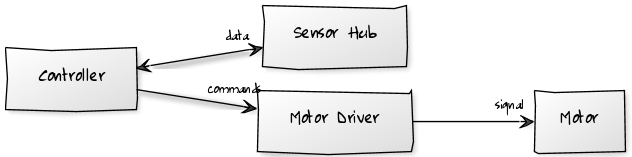
\includegraphics[width=4.0in] {Images/basic-uml.png}
        \caption{Basic system diagram}
        \label{Basic system diagram}
\end{figure}


\begin{figure}[h]
\centering
        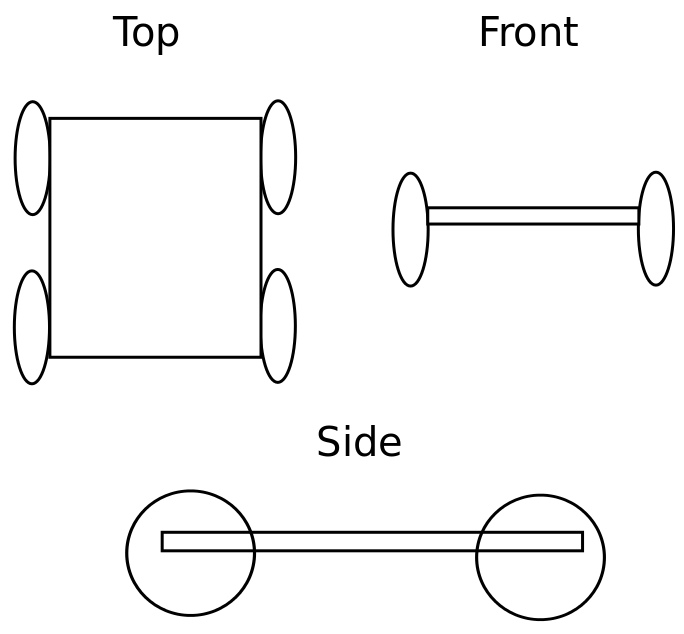
\includegraphics[width=4.0in] {Images/initial-design.png}
        \caption{Initial design}
        \label{Initial design}
\end{figure}

The central control unit will be a microcontroller for ease of interfacing directly with hardware as well as keeping power consumption down.  This controller will interface with both a motor control system and the various sensors required to detect objects in the environment around the robot.

\section{Justifications}
The various components that the project will need to come together into a finished product have many options.
\subsection{Materials}
I considered several materials for the robot chassis to be built of.
\begin{itemize}
\item Wood
\\This would be the easiest material to make the chassis from as it is very cheap, easy to cut into the intended shape and easy to mount components on with either adhesive, nails or screws.  Also the fact that it does not conduct electricity will help when mounting circuit boards to it.

\item Plastic
\\The lightest option.  Good due to its low weight but may not be as strong as wood or a metal option and could bend or snap under the load of heavier components such as motors or a large power source.  It can be more expensive than wood to aquire.  There is a higher difficulty in cutting it into the desired shapes.  It is also non-conductive, again useful to mount electronic components to.

\item Steel
\\A stronger material that can withstand a much heavier load, but is itself rather heavy compared to wood or plastic.  This extra base weight before adding anything else will put more strain onto the motors used to drive the robot and may even need to use more powerfull motors because of this extra weight.  It is a very conductive material which means that a non-conductive mounting platform will also be needed to mount electronic components as to avoid damaging them.

\item Aluminium
\\A much lighter metal than steel, but still much heavier than wood or plastic or the same thickness.  It can also take heavier loads than wood or plastic but it also much more difficult to cut.  Again aluminium is a very conductive material meaning that a non-conductive mounting platform will be needed.  It can also be used as a heat sink for the components that can get very hot such as the motor drivers or the motors themselves.

\end{itemize}

Aluminium seems to be the best all round choice being strong but not as heavy as steel.  It can act as a heat sink if the motors are mounted directly to it.  It is also not very expensive to buy in small amounts.
\\In addition to the aluminium base I have decided to use plastic for mounting components to the base.

\subsection{Actuators}
Actuators are motors used for controlling movement of a system.
\begin{itemize}
\item Servo
\\Typical servos are a motor and a gearbox with a potentiometer, a voltage divder in this case used to determine how far a motor has turned, for feedback.  These motors are great for controling such things as the direction of sensors or moving very light devices.  Servos are low voltage and as such do not have much strength, they are typicaly not good for driving larger equipment.  Also most servos only turn up to 180 degrees or 360 degrees, normaly they do not turn continuously but can eb modified to do so at the cost of losing the feedback of how far the motor has turned.

\item DC Motor
\\Direct current motor has a very simple operation.  Apply current to one side of the motor to make it turn, reverse the direction of the current to reverse the direction the motor turns.  Changing the speed of these motors is simple, either change the voltage, keeping it within the devices tollerences, or turn the current supplied to the motor on and off at high speed where how fast it it alternated determines the speed of the motor.  Typicaly these motors are attached to a gearbox to gain more torque to drive much higher loads.  Optical rotary encoders can be used to detemrine how much the motors have turned and how fast.

\item Steppers
\\Stepper motors use an internal gear and a ring of magnets.  These magnets pull the gear into position, powering the magnets in sequence will turn the motor.  Each part of this cycle is called a step.  This means that a single step is a know amount of rotation.  Using this type of motor means that you can accuratly turn whatever is attached to the motor shaft a known amount without any addition measuring equipment, although it may be used to verify that it has in fact moved the amount expected

\end{itemize}

I have chosen to use stepper motors due to the ability to control the amount and speed of rotation with more accuracy than the alternatives.  Stepper motors do come in high torque version which may be needed for this project as the chassis is made of metal.

\subsection{Sensors}

\begin{itemize}
\item LDR
\\An LDR is a light dependant resistor.  A small resistor that changes its resistance depending on how much light it is exposed to.  This could be used to detect if the robot is very close to bumping into an object and avoid it as the object would shadow some of the light from getting to the resistor, like a bump skirt.

\item Camera
\\A camera could be used to detect objects in front of it using various image processing techniques.  This method is good because it can potentialy map a relatively large area in a single image.  On the other hand it requires more processing to do, which can be slow and result in having colided into an object or be stuck in a tight space before it has finished processing.  I could use a more powerful processor to overcome this but it adds complexity, cost and power consumption.

\item Infra Red
\\Used to detect distance from an object.  Am emiter and a reciever pair linked to work like the light dependant resistor but using infra red instead of normal visible light.  Depending on the intensity of infra red picked up be the reciever it can be used to determine the distance from the source of the reflection.  Ambient infra red can effect readings.

\item Sonar
\\Again an emiter systle approach.  It emits and ultrasonic wave to bounce off of whatever surface is in front of it.  The time taken from emiting the wave until recieving the wave detemrines how far away the object is.  This method comes with its drawbacks.  Due to how sound waves behave when they interact with the environment by bouncing off of it.  If the surface is angled or curved the sound can bounce away from the reciever, either not reaching it at all giving the possible false reading that there is nothing in front of it, or it could bounce off of multiple surfaces back to the reciever giving a false reading that an object is there but further away due to the sound taking longer than it should have to reach the reciever.

\end{itemize}
A combination of both sonar and infra red logicaly seems like a good idea.  One can compensate for the others weaknesses.  Use the sonar to compensate for ambiant infra red and the infra red can be used to compensate for sonar bouncing around the environment.  Hopefully this will reduce the number of false readings produced.
\section{User Interface}

\section{Other relevant sections}
